
\documentclass[paper=a4, 
               fontsize=11pt, 
               footinclude=true,
               headinclude=true]{scrreprt}

%%%%% Paquetes
\usepackage[linedheaders, parts, pdfspacing, dottedtoc]{classicthesis}
\usepackage[left=1in, right=1in, top=1in, bottom=1in]{geometry}
\usepackage[utf8]{inputenc}
\usepackage[spanish]{babel}
\usepackage{parskip}
\usepackage{amsmath}
\usepackage{amsfonts}
\usepackage{amssymb}
\usepackage{graphicx}
\usepackage{tikz}
\usepackage{cite}

%%%%% Comandos general %%%%%
\newcommand{\Conjunto}[1]{\boldsymbol{\mathcal{#1}}}
\newcommand{\Estimado}[1]{\boldsymbol{\widehat{#1}}}

%%%%% Tikz %%%%%
\usetikzlibrary{shapes.geometric, shapes.multipart, backgrounds, fit, arrows}

\tikzstyle{flecha} = [thick,->,>=stealth]

\tikzstyle{data} = [trapezium, 
                    rounded corners,
                    trapezium stretches=true,
                    trapezium left angle=70, 
                    trapezium right angle=110, 
                    minimum width=2cm, 
                    minimum height=1cm, 
                    text centered, 
                    draw=black, 
                    fill=blue!30]

\tikzstyle{proceso} = [rectangle split,
                       rectangle split parts=2,
                       rectangle split part fill={red!30,blue!20},
                       rounded corners,
                       draw=black, 
                       minimum width=2cm, 
                       minimum height=1cm,
                       text centered,
                       text width=3.5cm,
                       inner sep=2pt]

\tikzstyle{proceso1} = [rectangle, 
                        rounded corners, 
                        minimum width=2cm, 
                        minimum height=1cm,
                        text centered, 
                        draw=black, 
                        fill=red!30]

\tikzstyle{contenedor} = [rectangle,
                          draw=black,
                          dashed,
                          inner sep=0.28cm, 
                          rounded corners,
                          fill=cyan!30!gray!20,
                          minimum height=4cm]

\tikzstyle{Fold_Split} = [rectangle, 
                          rounded corners, 
                          minimum width=1.5cm, 
                          minimum height=0.5cm,
                          text centered,
                          fill=white]

\tikzstyle{Fold1} = [rectangle, 
                     rounded corners, 
                     minimum width=1.5cm, 
                     minimum height=0.75cm,
                     text centered, 
                     draw=black, 
                     fill=blue!20]

\tikzstyle{Fold2} = [rectangle, 
                     rounded corners, 
                     minimum width=1.5cm, 
                     minimum height=0.75cm,
                     text centered, 
                     draw=black, 
                     fill=red!20]

\begin{document}


\begin{titlepage}

\begin{center}
\large

\begingroup
\color{Maroon}\spacedallcaps{El uso de modelos gráficos probabilísticos en predicción. Una aplicación con datos sobre la secuenciación genómica para detectar cáncer de cerebro} \\ \bigskip 
\endgroup

\spacedlowsmallcaps{DC} 

\end{center}

\end{titlepage}

\tableofcontents


\chapter{Introducción}

\section{Objetivos}

En este trabajo se explora el uso de modelos gráficos probabilísticos para el objetivo de predicción (clasificación supervisada) a partir de datos sobre las principales expresiones genómicas de las encimas asociadas a la ``vía de las kinureninas'' (KP, kynurenine pathway). Además, se exploran diferentes métodos (regresión logística, análisis de discriminante, maquina de soporte vectorial, etc.) para comparar los resultados en términos de poder predictivo.

El proyecto ``UCSC Xena'' \cite{Goldman} pone a disposición las bases de datos unidas sobre secuenciación genómica de diferentes proyectos para el análisis del cáncer.

Una de las bases de datos más usadas y que es la que se considera usar en este trabajo está disponible con el nombre ``A combined cohort of TCGA, TARGET and GTEx samples'' y es el resultado del preprocesamiento para poder unir las bases de datos que se describe en \cite{Vivian}.

\section{Motivación}

La motivación de este trabajo surge a partir del objetivo de detectar personas con tumores cerebrales de bajo grado y tumores cerebrales altamente agresivos de manera oportuna y certera a través de procesos que no impliquen una intervención quirúrgica.

La discusión de este trabajo está centrada en la interpretación de los resultados, las limitaciones de los métodos explorados así como de los datos utilizados, posibles mejoras dentro de los métodos explorados y las posibles implicaciones que tendría este trabajo para el planteamiento de futuros trabajos y protocolos de investigación.

\chapter{Metodología}

\section{Aprendizaje supervisado}

Consideremos un conjunto de datos que consta de $n$ observaciones, representadas a través de $p$ variables distintas, es decir:

\begin{equation*}
    \Conjunto{X} = \Big\{\boldsymbol{x}_i \in \mathbb{R}^p | i = 1,...,n \Big\}
\end{equation*}

Al conjunto $\boldsymbol{\mathcal{X}}$ le llamaremos el conjunto de datos de entrada y a sus elementos como observaciones. Es común utilizar una representación matricial del conjunto $\boldsymbol{\mathcal{X}}$ de tal forma que los datos son representados como valores $x_{ij}$, donde $i \in \{1,...,n\}$ hace referencia a la $i$-ésima observación, mientras que $j \in \{1,...,p\}$ indica la $j$-ésima variable de cada observación, es decir:

\begin{equation*}
    \Conjunto{X} = 
    \begin{pmatrix}
        x_{11} & \cdots & x_{1p} \\
        \vdots & \ddots & \vdots \\
        x_{n1} & \cdots & x_{np}
    \end{pmatrix}
\end{equation*}

Ahora supongamos que cada elemento $\boldsymbol{x}_i \in \Conjunto{X}$ esta etiquetado por un único valor $y_i \in \Conjunto{Y}$. Al conjunto $\Conjunto{Y}$ le llamaremos el conjunto de etiquetas y en general se pueden distinguir dos casos:

\begin{itemize}
    \item \textit{Regresión}: Cuando el conjunto $\Conjunto{Y}$ es un subconjunto de $\mathbb{R}$.
    \item \textit{Clasificación}: Cuando el conjunto $\Conjunto{Y}$ toma una cantidad finita de valores $\{\mathrm{C}_1,...,\mathrm{C}_k\}$ con $k \in \mathbb{N}$. A los elementos $\mathrm{C}_1,...,\mathrm{C}_k$ les llamaremos \textit{clases}.
\end{itemize}

Al conjunto conformado por la relación entre los datos de entrada $\Conjunto{X}$ y de salida $\Conjunto{Y}$ le llamaremos el conjunto de datos etiquetados y lo denotaremos como $\Conjunto{D}$, es decir: 

\begin{equation*}
    \Conjunto{D} = \Big\{(y_i, \boldsymbol{x}_i) \in \mathbb{R}^{p+1} | i = 1,...,n \Big\}
\end{equation*}

O de manera matricial como:

\begin{equation*}
    \Conjunto{D} = 
    \begin{pmatrix}
        y_{1}  & x_{11} & \cdots & x_{1p} \\
        \vdots & \vdots & \ddots & \vdots \\
        y_{n}  & x_{n1} & \cdots & x_{np}
    \end{pmatrix}
\end{equation*}

El aprendizaje supervisado es un enfoque dentro del campo del aprendizaje automático (\textit{machine learning}), donde se entrena un modelo utilizando un conjunto de datos etiquetados $\Conjunto{D}$ con el propósito de realizar predicciones para \textbf{nuevas observaciones}. En el contexto del aprendizaje supervisado, diremos que una observación es nueva cuando no se dispone de información previa acerca de la etiqueta asociada a dicha observación. Denotaremos al conjunto de nuevas observaciones como $\Conjunto{X}^*$, y a sus elementos como $\boldsymbol{x}^*$.

Un algoritmo de aprendizaje supervisado $\mathcal{A}_{\boldsymbol{\lambda}}$ es una función que mapea un conjunto de datos etiquetados $\Conjunto{D}$ a una función $\widehat{f}$, es decir:

\begin{alignat*}{1}
  \mathcal{A}_{\boldsymbol{\lambda}}: \Conjunto{D} &\longrightarrow f \\
               \Conjunto{D} &\longmapsto \widehat{f}
\end{alignat*}

A su vez la función $\widehat{f}$ mapea nuevas observaciones $\boldsymbol{x}^*$ a etiquetas dentro del conjunto $\Conjunto{Y}$, llamaremos a estas etiquetas como \textbf{predicciones} y las denotaremos como $\widehat{y}$, es decir:

\begin{alignat*}{1}
  \widehat{f}: \Conjunto{X}^* &\longrightarrow \Conjunto{Y} \\
                 \boldsymbol{x}^* &\longmapsto \widehat{y}
\end{alignat*}

A la función $\widehat{f}$ la llamaremos modelo ajustado y es el resultado de un proceso de \textbf{aprendizaje} siguiendo el algoritmo $\mathcal{A}_{\boldsymbol{\lambda}}$. 

Es importante mencionar que en varios casos un algoritmo puede depender de ciertas configuraciones que son establecidas antes de comenzar con el proceso de entrenamiento, llamaremos a estas configuraciones como hiperparámetros y denotaremos al conjunto de posibles hiperparámetros como $\Lambda$.

\begin{figure}[h]
    \centering
    \begin{tikzpicture}[node distance=2cm]
        \node (Data) [data] {$\Conjunto{D}$};
        \node (Split) [proceso1, right of=Data, xshift=1cm] {Split};
        \node (Validation) [data, right of=Split, xshift=1cm] {$\Conjunto{D}_{\text{Val}}$};
        \node (Train) [data, above of=Validation] {$\Conjunto{D}_{\text{Train}}$};
        \node (Test) [data, below of=Validation, yshift=-1cm] {$\Conjunto{D}_{\text{Test}}$};
        \node (Algoritmo) [proceso, right of=Validation, xshift=2cm] {$\mathcal{A}$
            \nodepart{two} Estimación: $\Estimado{\beta}$ \\ 
                           Selección: $\Estimado{\lambda}$};
        \node (Prediccion) [proceso, right of=Test, xshift=2cm] {$\widehat{f}$ 
            \nodepart{two} Predicciones: $\widehat{f}(\boldsymbol{x}^*)$};
        \node (Evaluacion) [proceso, below of=Prediccion] {$\mu$ 
            \nodepart{two} Evaluación: $\mu(y,\widehat{y})$};

        \begin{scope}[on background layer]
            \coordinate (aux1) at ([yshift=3mm]Train.north);
            \node (Aprendizaje) [contenedor, fit=(aux1) (Validation)(Algoritmo)] {};
            \node at (Aprendizaje.north) [fill=white,draw,font=\fontsize{10}{0}\selectfont] {\textbf{Aprendizaje}};
        \end{scope}

        \begin{scope}[on background layer]
            \coordinate (aux2) at ([yshift=3mm]Prediccion.north);
            \node (Eval) [contenedor, fit=(aux2) (Test)(Evaluacion)] {};
            \node at (Eval.north) [fill=white,draw,font=\fontsize{10}{0}\selectfont] {\textbf{Evaluación}};
        \end{scope}

        \draw [flecha] (Data) -- (Split);
        \draw [flecha] (Split) -- (Validation);
        \draw [flecha] (Split) |- (Train);
        \draw [flecha] (Split) |- (Test);
        \draw [flecha] (Validation) -- node[above] {$\boldsymbol{\lambda}$} (Algoritmo);
        \draw [flecha] (Train) -| node[above] {$\boldsymbol{\beta}$} (Algoritmo);
        \draw [flecha] (Algoritmo) -- (Prediccion);
        \draw [flecha] (Test) -- node[above] {$\boldsymbol{x}^*$} (Prediccion);
        \draw [flecha] (Prediccion) -- node[right] {$\widehat{y}$} (Evaluacion);
        \draw [flecha] (Test) |- node[below] {$y$} (Evaluacion);
    \end{tikzpicture}
    \caption{Proceso general para la implementación de un modelo de aprendizaje}
    \label{fig:Fig1}
\end{figure}


\subsection{Repeated k-Fold Cross-Validation} \label{R K-CV}

\begin{figure}[h]
    \centering
    \begin{tikzpicture}
        \node (S1_F1) [Fold1] {Test};
        \node (S1_F2) [Fold2, right of=S1_F1, xshift=0.6cm] {Train};
        \node (S1_F3) [Fold2, right of=S1_F2, xshift=0.6cm] {Train};
        \node (S1_F4) [Fold2, right of=S1_F3, xshift=0.6cm] {Train};
        \node (S1_F5) [Fold2, right of=S1_F4, xshift=0.6cm] {Train};

        \node (S2_F1) [Fold2, below of=S1_F1, yshift=0.1cm] {Train};
        \node (S2_F2) [Fold1, right of=S2_F1, xshift=0.6cm] {Test};
        \node (S2_F3) [Fold2, right of=S2_F2, xshift=0.6cm] {Train};
        \node (S2_F4) [Fold2, right of=S2_F3, xshift=0.6cm] {Train};
        \node (S2_F5) [Fold2, right of=S2_F4, xshift=0.6cm] {Train};

        \node (S3_F1) [Fold2, below of=S2_F1, yshift=0.1cm] {Train};
        \node (S3_F2) [Fold2, right of=S3_F1, xshift=0.6cm] {Train};
        \node (S3_F3) [Fold1, right of=S3_F2, xshift=0.6cm] {Test};
        \node (S3_F4) [Fold2, right of=S3_F3, xshift=0.6cm] {Train};
        \node (S3_F5) [Fold2, right of=S3_F4, xshift=0.6cm] {Train};

        \node (S4_F1) [Fold2, below of=S3_F1, yshift=0.1cm] {Train};
        \node (S4_F2) [Fold2, right of=S4_F1, xshift=0.6cm] {Train};
        \node (S4_F3) [Fold2, right of=S4_F2, xshift=0.6cm] {Train};
        \node (S4_F4) [Fold1, right of=S4_F3, xshift=0.6cm] {Test};
        \node (S4_F5) [Fold2, right of=S4_F4, xshift=0.6cm] {Train};

        \node (S5_F1) [Fold2, below of=S4_F1, yshift=0.1cm] {Train};
        \node (S5_F2) [Fold2, right of=S5_F1, xshift=0.6cm] {Train};
        \node (S5_F3) [Fold2, right of=S5_F2, xshift=0.6cm] {Train};
        \node (S5_F4) [Fold2, right of=S5_F3, xshift=0.6cm] {Train};
        \node (S5_F5) [Fold1, right of=S5_F4, xshift=0.6cm] {Test};

        \node (F1) [Fold_Split, above of=S1_F1, yshift=-0.2cm] {Fold 1};
        \node (F2) [Fold_Split, right of=F1, xshift=0.6cm] {Fold 2};
        \node (F3) [Fold_Split, right of=F2, xshift=0.6cm] {Fold 3};
        \node (F4) [Fold_Split, right of=F3, xshift=0.6cm] {Fold 4};
        \node (F5) [Fold_Split, right of=F4, xshift=0.6cm] {Fold 5};

        \node (S1) [Fold_Split, left of=S1_F1, xshift=-0.6cm] {Split 1};
        \node (S2) [Fold_Split, left of=S2_F1, xshift=-0.6cm] {Split 2};
        \node (S3) [Fold_Split, left of=S3_F1, xshift=-0.6cm] {Split 3};
        \node (S4) [Fold_Split, left of=S4_F1, xshift=-0.6cm] {Split 4};
        \node (S5) [Fold_Split, left of=S5_F1, xshift=-0.6cm] {Split 5};
    \end{tikzpicture}
    \caption{k-Fold Cross-Validation}
    \label{fig:Fig2}
\end{figure}


\subsection{Métricas de desempeño} \label{MD}

\subsection{Algoritmos de clasificación} \label{AC}

\subsubsection{Regresión Logística} \label{RL}

\subsubsection{Análisis de Discriminante Lineal} \label{ADL}

\subsubsection{Análisis de Discriminante Cuadrático} \label{ADC}

\subsubsection{Máquina de Soporte Vectorial} \label{MSV}

\subsubsection{Bosques Aleatorios} \label{BA}

\subsubsection{Redes Neuronales} \label{RN}

\subsection{Modelos gráficos probabilísticos en predicción} \label{MGP}



\chapter{Caso práctico} \label{CP}
\section{Datos}

\section{Análisis exploratorio}

\begin{figure}[h]
    \centering
    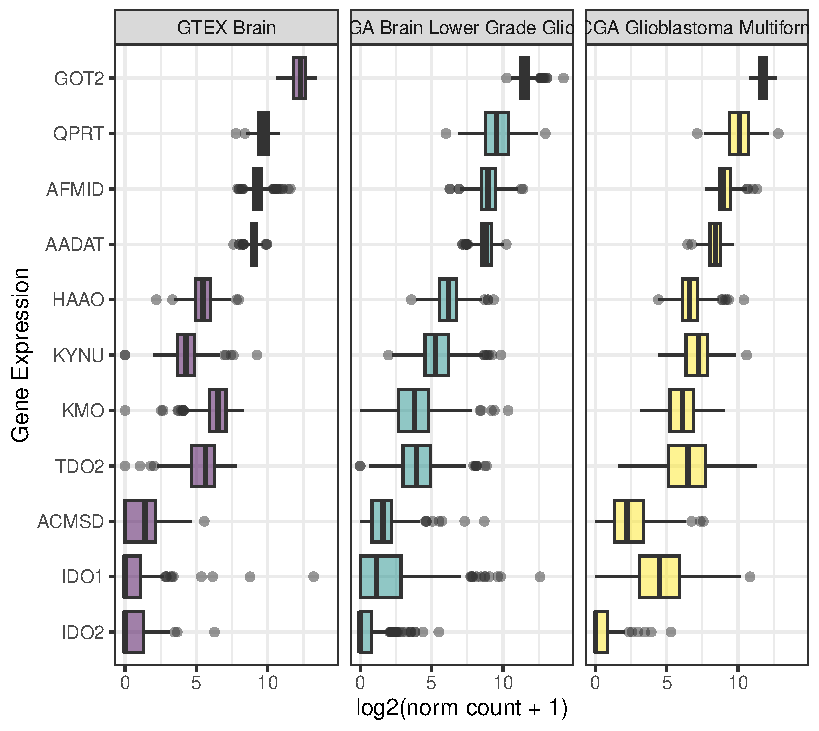
\includegraphics{Imagenes/Rplot.pdf}
    \caption{Texto...}
    \label{fig:Fig}
\end{figure}

En la Figura \ref{fig:Fig1} se puede observar...

\section{Estimación del poder predictivo}


\chapter{Discusión y conclusiones}
\section{Análisis de los resultados}

\section{Limitaciones y posibles mejoras}



\chapter{Anexo}

\section{Sobre el código utilizado}

El código que se utilizó para el desarrollo de este trabajo puede ser consultado en el siguiente \href{https://github.com/DanielCuaxiloa/Tesis}{repositorio} en GitHub.

\nocite{ISL, GMWR, epskamp2018tutorial, Gonzalo}

\bibliographystyle{apalike}
\bibliography{referencias}

\end{document}